%%==================================================
%% chapter01.tex for BIT Master Thesis
%% modified by yang yating
%% version: 0.1
%% last update: Dec 25th, 2016
%%==================================================
\chapter{seL4介绍}
\label{chap:seL4_intro}
\section{seL4的发展历史及主要特征}
seL4是一款具有创新性和里程碑意义的微内核。seL4项目始于2006年的澳大利亚悉尼大学,其目标是创建一个经过形式化验证的微内核,从而确保内核的安全性和可靠性。在2009年,seL4正式发布了针对arm 11处理器的功能正确性的形式化证明,是全球首个经过完整形式化验证的微内核。在2014年,seL4正式开源,得到了来自开源社区的广泛关注,seL4的生态蓬勃发展。在接下来的几年里,seL4陆续完成了对不同CPU和不同指令集架构的验证和支持、虚拟化支持等,并在应用生态领域有了丰富的支持。

seL4的设计遵循一下几个原则\cite{sel4DesignPrinciples}: 
\begin{itemize}
  \item Verification:截止目前(2025年3月),seL4依然是第一个经过形式化验证的内核,形式化验证对 seL4 是个坚持不懈的努力目标,为了验证方便,禁止在内核里并发处理,不允许在内核态的大部分场景里再次发生中断。
  \item Minimality:一方面最小化原则是 L4 家族的根本设计理念,另一方面,最小化也是方便 seL4 做形式化验证的重要条件,seL4 内核除了中断控制器、定时器、MMU 相关的一点硬件驱动代码,其它驱动都在用户空间运行。
  \item Policy freedom:seL4 对于大部分资源分配策略都移到了用户态进行定制,通过Capabiltiy进行管理。
  \item Performance:虽然极度关注安全、可形式化验证,seL4 着重对热点路径的优化,因此依然有着突出的性能优势。
  \item Security:seL4在安全性设计上遵循最小权限原则(Least privilege),通过capability机制来保证任何组件只拥有完成其工作所需的权限。
\end{itemize}

\section{seL4的基本组成}

如图\ref{fig:seL4_frramework}所示,seL4基本采用分层的设计理念,在内核态保留了虚拟地址管理(VMM),进程间通信(IPC)、通知机制(Notification)、任务调度(Scheduler)和中断管理(Interrupt Manager),同时在内核态提供能力访问控制(Capability)来进行权限管理。驱动程序和大部分系统服务(如网络协议栈和文件系统等)运行在用户态,应用程序通过IPC请求系统服务,同时,硬件中断通过Notification传递给用户态驱动。

\begin{figure*}[htbp]
  \centering
  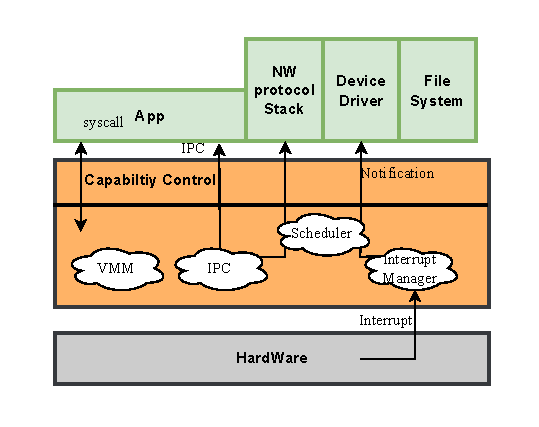
\includegraphics[width=0.75\textwidth]{figures/seL4_framwork.drawio.pdf}
  \caption{seL4的系统结构图}\label{fig:seL4_frramework}
\end{figure*}

\subsection{内核对象与Capability机制}

在 seL4 中,内核对象是操作系统内核所管理和操作的基本实体,是系统资源的软件抽象。内核通过维护内核对象的状态来维护系统状态。主要的内核对象如表\ref{tab:kernel_object}所示。

\begin{table*}[htbp]
  \centering
  \begin{tabular*}{1.0\textwidth}{@{\extracolsep{\fill}}ll}
  \toprule
    内核对象			&作用	 \\
  \midrule
    线程控制块(TCB)			&内核调度的基本单位,保存了用户任务运行所需的上下文。 \\
    能力空间(CSpace)			&访问能力的集合,维护了各个内核对象的访问能力和对应权限。	 \\
    地址空间(VSpace) &地址空间,维护了一段虚拟地址和物理地址的映射关系。	 \\
    物理页框(Frame)  &对应一个物理页,维护了物理页号和访问权限.\\
    端点(Endpoint)	&同步IPC的桥梁,维护了一个消息收发的状态机。 \\
    通知对象(Notification) &通知机制的桥梁,维护了一个通知状态位。\\
    无类型对象(Untyped)&物理内存管理的承载者,通过系统调用转化为其他内核对象。 \\
  \bottomrule
  \end{tabular*}
  \caption{seL4中的主要内核对象} \label{tab:kernel_object}
\end{table*}

内核对象无法直接被用户态访问,只能通过Capability机制将能力句柄(Capability handler)暴露给用户态,用户态在handler上调用系统调用来对内核对象进行访问。能力句柄是能力(Capability)的索引,在Capability中,内核维护了对应的内核对象地址以及对应的访问权限,当用户态在handler上发起系统调用时,内核会通过查找到相应的Capabiltiy并检查对应的权限,权限检查通过之后会根据地址对内核对象进行相应的操作。

Capabiltiy可以被转移和派生,转移之后原始的用户态进程就不再拥有对相应内核对象操作性的权限,而派生则保留了原始进程的权限,派生的Capabiltiy的权限是原始权限的子集,被派生的Capabiltiy可以进一步派生,由此在内核形成一个能力派生树(Capability Tree),为了保证可控性,父节点可以通过revoke操作随时回收子节点的能力。由此,seL4通过能力派生的形式递归地构建了整个系统的权限控制体系。

\subsection{内存管理}
seL4中将物理内存管理和虚拟内存管理分开。物理内存由用户态管理,而虚拟内存由内核态管理。

\begin{figure*}[htbp]
  \centering
  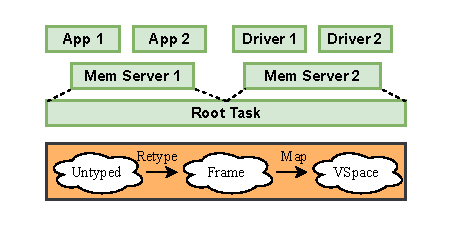
\includegraphics[width=0.75\textwidth]{figures/seL4_mm.drawio.pdf}
  \caption{seL4的内存管理}\label{fig:seL4_mm}
\end{figure*}

如图\ref{fig:seL4_mm}所示,在seL4中,有一类特殊的无类型内核对象Untyped,保存了未被分配的物理内存信息,用户态通过Retype系统调用将其转化为小的Untyped或者有类型的内核对象(如Frame)。内核在启动完成之后将所有的Untyped对象的Capabiltiy交给Root Task用户进程,Root Task将通过Retype或能力派生的形式对空闲的物理内存进行进一步分配,由此可见,seL4系统中的物理内存管理也是分布式递归管理的。

在seL4中,每个进程都包含了一个VSpace内核对象,对应一个根页表,维护了进程地址空间的映射关系,而用户态通过map/unmap系统调用将Frame内核对象和虚拟地址的映射关系修改到页表中。

\subsection{任务调度}
\label{sec:sel4_task}
在seL4中,线程是任务调度的基本单位和执行单元,每个线程包含了一组能力空间和一套执行上下文。进程的概念被弱化,通常情况下,我们将含有相同能力空间和地址空间的称为同一个进程,将进程抽象为资源分配的基本单位,因此在seL4中,进程只作为一个逻辑概念存在,内核的设计和实现只涉及到线程。

在seL4中,线程调度主要分为两类:优先级调度和抢占调度。优先级调度时机一般是某个任务时间片用完、或由于阻塞事件无法继续执行时,内核从优先级队列中取出最高优先级的队头任务进行调度执行。而抢占调度一般发生在同步IPC中,当某个线程的操作唤醒了另外一个线程,在不违反优先级调度原则的前提下,会优先插队调度。具体的同步IPC流程描述参考\ref{sec:sel4_ipc}。线程的状态转换图如\ref{fig:seL4_thread_state}所示。

\begin{figure*}[htbp]
  \centering
  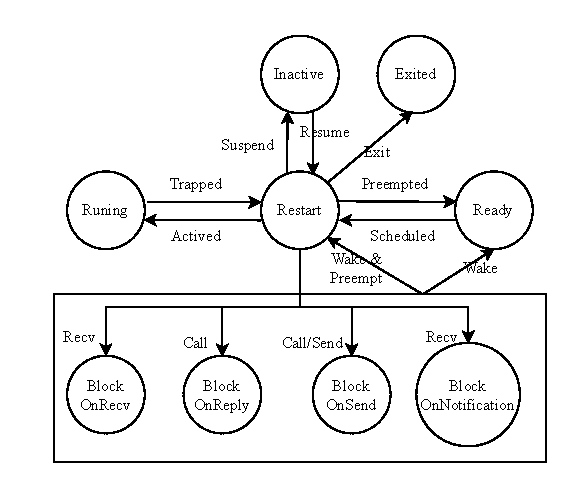
\includegraphics{figures/seL4_thread_state.drawio.pdf}
  \caption{seL4的线程状态转换}\label{fig:seL4_thread_state}
\end{figure*}

此外,seL4的MCS扩展还支持混合关键性系统(MCS)来进行实时性调度,内核通过时间片预留、动态调整和模式切换来保证任务的实时性。

\subsection{同步IPC和通知机制}
\label{sec:sel4_ipc}

seL4设计者认为系统中的大部分IPC都遵循客户端/服务器(C/S)架构,客户端线程发起请求后等待服务端线程接收请求并返回响应,在此之前,客户端进程会阻塞在一个名为Endpoint的内核对象上,相似的,服务端线程也会阻塞监听Endpoint对象,直到有请求到来。如\ref{fig:seL4_ipc_state}内核通过维护Endpoint状态和阻塞队列来维持通信的秩序。值得注意的是,在seL4中,同步IPC更像是任务调度的一部分,同步IPC可能会导致任务的切换,以客户端在OnRecv状态的Endpoint发起请求为例,在不违反优先级调度原则的前提下,内核会将阻塞队列中的服务端线程唤醒并切换执行(即\ref{sec:sel4_task}中的抢占调度),而将客户端线程阻塞并等待响应。

\begin{figure*}[htbp]
  \centering
  \includegraphics{figures/seL4_ipc_state.drawio.pdf}
  \caption{seL4的IPC相关内核对象状态转换}\label{fig:seL4_ipc_state}
\end{figure*}

由于同步IPC强制用户态以多线程的形式处理并发,因此seL4还支持非阻塞的通知机制,客户端线程非阻塞地通知接受线程,不会阻塞地等待服务端发起接收流程,由此解放了客户端线程,而服务端线程则依然要阻塞地接收客户端的信号,因此对于服务端来说依然是同步的流程。如\ref{fig:seL4_ipc_state}所示,与同步IPC类似,seL4通过在Notification内核对象中维护对象状态和一组信号字来实现通知机制,在相似的情况下也会导致任务的切换。

\subsection{中断管理与SMP支持}
seL4在中断管理与对称多处理机(SMP)支持方面也与主流内核有所区别,seL4为了保证内核行为的可预测性,在内核中屏蔽了所有外部中断,禁止内核中的中断抢占,这是由于seL4中的大部分内核任务都极其简短,因此停留在内核中(屏蔽中断)的时间非常少,不会过多地影响系统的实时性,而对于少量可能造成内核执行时间较长的系统调用,seL4在这些系统调用中插入了可抢占点,将内核的行为约束在可控范围内。

出于同样的目的,对于多CPU核心系统,seL4通过内核锁保证只有一个核心运行在内核态,避免了复杂的内核资源竞争,同时保证了内核行为的可预测性,大部分的系统调用都只会短暂停留在内核中,一般不会出现饥饿等待的情况,而对于少量可能造成内核执行时间较长的系统调用,seL4在流程中添加重启点,保存少量用于指示当前执行状态的信息,然后释放内核锁,等待下一次获取内核锁之后重启流程,以此避免饥饿等待的发生。

